\documentclass[]{SangerLibrary/sanger-present}
\usepackage{JML}
\usetikzlibrary{decorations.pathreplacing,calligraphy}
\graphicspath{{Images/}}

\usepackage{fp}
\usepackage{pgfplots}
\usepackage{siunitx}
% \usepackage[usedvipsnames]{xcolor}

\title{\Huge Under The Hood\\ {\footnotesize A Peek Inside the 'Black Box' of Machine Learning}}
\author{\large Jack Fraser-Govil}
\institute{The Wellcome Sanger Institute, Hinxton, UK}
\date{\small 18th May 2023}

\def\cuteB{-3}
\def\cuteWA{0}
\def\cuteWB{1}
\def\learn{0.01}
\newcommand\cute[5]
	{
		\def\cuteLabel{#5}
		\def\labelText{Not Cute}
		\ifnum\cuteLabel=1
			\def\labelText{Cute}
		\fi
		\node at ({#1},{#2}) {\includegraphics[width=2cm,height=2cm,keepaspectratio=true]{#3}};
		
		% \node at ({#1},{#2}) {#4 \highlight{}};
		\def\test{#4}
		\def\comp{\highlight}




		%%%PERCEPTRON IMPLEMENTED WITHIN IMAGE PLACEMENT
		\ifnum\test=\comp

			\FPeval{dot}{(\a) + (#1*(\b)) + (#2*(\c))}
			\def\cuteGuess{0}
			\pgfmathparse{\dot<0}

			%COMPUTE ASSIGNED VALUE
			\ifnum\pgfmathresult=0
				\def\cuteGuess{1}
			\fi
			\def\guessText{Not Cute}
			\if\cuteGuess1
				\def\guessText{Cute}
			\fi
			
			%DRAW COLOUR
			\def\highcolour{\wrongcolour}
			\ifnum\cuteGuess=\cuteLabel
				\def\highcolour{\rightcolour}
			\else

				%%%UPDATE WEIGHTS IF GUESSED WRONG
				\xdef\updated{1}
				\FPeval{bup}{(\cuteB) + ((\cuteLabel)-(\cuteGuess))*(\learn)}
				\FPeval{waup}{(\cuteWA) + ((\cuteLabel)-(\cuteGuess))*(\learn)*(#1)}
				\FPeval{wbup}{(\cuteWB) + ((\cuteLabel)-(\cuteGuess))*(\learn)*(#2)}
				\xdef\cuteB{\bup}
				\xdef\cuteWA{\waup}
				\xdef\cuteWB{\wbup}
			\fi
			\fill[\highcolour,opacity=0.2] ({#1},{#2}) circle (1.3);
			% \node[red] at ({#1},{#2}) {\a +#1* \b + #2 * \c = \dot};
			
			\node at ({#1},{#2+1.1}) {\tiny Labelled: \labelText, Guess \guessText};
		\else
			% \node at ({#1},{#2-1.1}) {\tiny \labelText};
		\fi
		
	}
% \setbeamercolor{background canvas}{bg=SangerLight}
% \logo{\SangerLogoBlack}
\def\highlight{0}
\def\rightcolour{green!70!black}
\def\wrongcolour{red!70!black}
\def\highcolour{\rightcolour}
\newcommand\animals{
	\cute{0.7}{3.5}{mouse}{1}{1}
	\cute{2}{6}{rabbit}{2}{1}
	\cute{6}{5.7}{dog}{3}{1}
	\cute{4}{5.8}{cat}{4}{1}
	\cute{9}{5.5}{lion}{5}{0}
	\cute{10}{1}{whale}{6}{0}
	\cute{7}{2.7}{warthog}{7}{0}
	\cute{1.7}{1}{molerat}{8}{0}
	\cute{4}{2}{ayeaye}{9}{0}
	\cute{0.1}{0.1}{ant}{10}{0}
}

\newcommand\confusing{
	\cute{2}{6}{rabbit}{1}{1}
	\cute{9}{5.5}{lion}{2}{0}
	\cute{10}{1}{whale}{3}{1}
	\cute{0.1}{0.1}{ant}{4}{0}
}

\begin{document}
	\maketitlepage

	\begin{frame}{Why bother?}

		% \begin{itemize}
		% 	\item What is Machine Learning?
		% 	\item Perceptrons
		% 	\item Upgrades: The Multilayer Perceptron
		% 	\item Introduction to optimisation
		% 	\item Batching
		% 	\item Optimisation \& Overfitting
		% 	\item Extensions to MLP: convnets etc. 
		% \end{itemize}

		In a world with dozens of pre-built ML tools....why bother studying the fundamentals?

		\pause In a word...
		\pause\begin{center}
			\LARGE FOLKLORE
		\end{center}
		% \pause Might get you where you need to go...but often leads you astray
	\end{frame}
	\begin{frame}{ML Folklore}
		\begin{itemize}
			\pitem ADAM vs AdaGrad?
			\pitem Softplus vs ReLu vs Leaky ReLu vs Sigmoid?
			\pitem Cross-Entropy vs Least Squares?
			\pitem Validation set magic numbers
		\end{itemize}
	\end{frame}

	\begin{frame}{Basic Decision Making: Defining Cuteness}

		
		\begin{center}
			\def\w{8}
			\begin{tikzpicture}

				\animals
				\draw[->] (0,0)--node[below]{Size} (10,0);
				\draw[->] (0,0)--node[left]{Fur} (0,6);
				\pause \draw[dashed] (0,1)--node[above,rotate=30] {\textbf{Cute}} node[below,rotate=30] {\textbf{Not Cute}} (8,6);

			\end{tikzpicture}
		\end{center}

	\end{frame}

	\begin{frame}{In maths...}
		Let $\vec{x}$ be the `feature vector', $\vec{x} = \begin{pmatrix}1 \\ \text{size} \\ \text{fur}\end{pmatrix}$, and $\vec{w} = \begin{pmatrix} w_0 \\ w_1 \\ w_2 \end{pmatrix}$ be our `weights':


		\pause The Perceptron algorithm is:

		\begin{spalign}
			{\mathcal{P}_{\vec{w}}}(\vec{x}) =  \begin{cases} 1 \text{ (cute)} & \text{ when }\vec{w} \cdot \vec{x} > 0
				\\
				0 \text{ (not cute)}& \text{else}\end{cases}
		\end{spalign}


		\pause Therefore $\vec{w}$ defines a \textit{line} which divides our 2D space -- Perceptron simply splits the region into two $\to$ though can pull some fancy tricks.
	\end{frame}

	\begin{frame}{Training Perceptron}
		Training = finding the \textit{best} $\vec{w}$
		
		\pause Perceptron algorithm loops over a labelled `training set', where the known cuteness of $j$ is $C_j$

		\begin{equation}
			\vec{w} \to \vec{w} + r \left(C_j - \mathcal{P}_{\vec{w}}(\vec{x}_j) \right)\vec{x}_j
		\end{equation}
		\pause In words
		
		{\centering \it For each element in the set, if I guess wrong ($C_j \neq \mathcal{P}_j$), move $\vec{w}$ by a small amount ($r$) to make me less wrong.}
	\end{frame}



	\newcommand\trainingFrame[1]
	{
		\def\highlight{#1}
		% \def\highcolour{#2}
		\def\a{\cuteB}
		\def\b{\cuteWA}
		\def\c{\cuteWB}
		\FPeval{M}{round(0 - \b/(\c+0.001),1)}
		\FPeval{C}{round(0 - \a/(\c+0.001),1)}
		\FPeval{burst}{(7-\C)/(\M+0.001)}

		% \FPeval{mval}{min(10,\burst)}
		% \pgfmathparse{\mval<0}
		% \ifnum\pgfmathresult=1
		% 	\FPeval{burst}{(0-\C)/(\M+0.001)}

		% 	\FPeval{mval}{max(0,min(10,\burst))}
		% \fi
		% \ifnum\mval=0
		% 	
		% \fi
		% \FPeval{\M}{-(\b)/((\c)+0.00000001)}
		% \FPeval{\C}{-(\a)/((\c)+0.000000001)}		
		\begin{frame}{Training Perceptron}

		
			\begin{center}
				\def\w{8}
				\begin{tikzpicture}
					\useasboundingbox (0,0) rectangle (12,7.5);
					\node at (11,7) {\large $\vec{w} = (\num[round-mode=places,round-precision=2]{\a},\num[round-mode=places,round-precision=2]{\b},\num[round-mode=places,round-precision=2]{\c})$};
					\animals
					\draw[->] (0,0)--node[below]{Size} (10,0);
					\draw[->] (0,0)--node[left]{Fur} (0,6);
					\def\theta{0}
					
					\draw[ultra thick,dashed,black] (0,{\C})--(14,{14*\M+\C});
					
					% \node at (4,3) {\small \M --- \C};
					% \node at (4,2) {\mval-- \burst};
				\end{tikzpicture}
			\end{center}
	
		\end{frame}
	}
	
	\def\cuteB{-1}
	\def\cuteWA{0.5}
	\def\cuteWB{0.145}
	\def\learn{0.017}
	\trainingFrame{-1}
	\foreach \q in {1,...,10}
	{
		\def\updated{0}
		\foreach \animal in {1,...,10}
		{
			\trainingFrame{\animal}
			% \node at ({0.1*\loop},{0.2*\animal}) {\loop,\animal};
		}
		\if\updated0
			\breakforeach
		\fi
	}

	% \begin{frame}{The Mk. 1 Perceptron}
	% 	\begin{center}
	% 		\begin{tikzpicture}
	% 			\draw[ultra thick,->] (-6,0)--node[above]{20$\times$20 pixel image} (-3,0);

	% 			\node at (0,0)	{\includegraphics[keepaspectratio=true,height=0.7\paperheight]{perceptronReal}};

	% 			\draw[ultra thick,->] (3,0)--node[above]{$0\leq x \leq 1$}	(6,0);%%keep image in center
	% 			\draw[ultra thick,dashed,->,red!70!black]   (-4,-3)--node[pos=0,below] {Input layer} (-0.5,-2);

	% 			\draw[ultra thick,dashed,->,red!70!black]  (5,3)--node[pos=0,above] {Weights (potentiometers)} (1.9,1);
	% 		\end{tikzpicture}
		
	% 	\end{center}

	% 	\pause \small We'll come back to the wisdom of using a perceptron for image recognition....
	% \end{frame}

	\begin{frame}{Getting clever....}
		Can get non-straight lines by using $(x,x^2,x^3,y,xy,\cos(y^2 x^3),\hdots)$

		\pause But needs pre-defined user input!
	\end{frame}

	\begin{frame}{Major limitations....}
		\begin{center}
		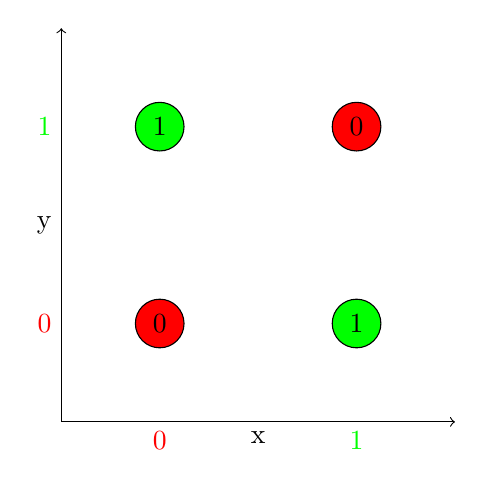
\begin{tikzpicture}
			\draw[->] (0,0)--node[below]{x} (5,0);
			\draw[->] (0,0)--node[left]{y} (0,5);

			\node[anchor=north] at ({5.0/4},0) {\color{red} 0};
			\node[anchor=north] at ({5-5/4},0) {\color{green} 1};
			\node[anchor=east] at (0,{5.0/4}) {\color{red} 0};
			\node[anchor=east] at (0,{5-5/4}) {\color{green} 1};

			\node[draw,circle,fill=red] at ({5.0/4},{5.0/4}){0};
			\node[draw,circle,fill=red] at ({5-5.0/4},{5-5.0/4}){0};
			\node[draw,circle,fill=green] at ({5.0/4},{5-5.0/4}){1};
			\node[draw,circle,fill=green] at ({5-5.0/4},{5.0/4}){1};
		\end{tikzpicture}
	\end{center}
	\pause Can \textbf{never} be solved by perceptron
	\end{frame}

	\newcommand\cec[1]{{\vec{#1}}}
	{
	\nologo
	\begin{frame}{The Multilayered Perceptron}
		% Let's try chaining lots of pecreptrons together.....
		
		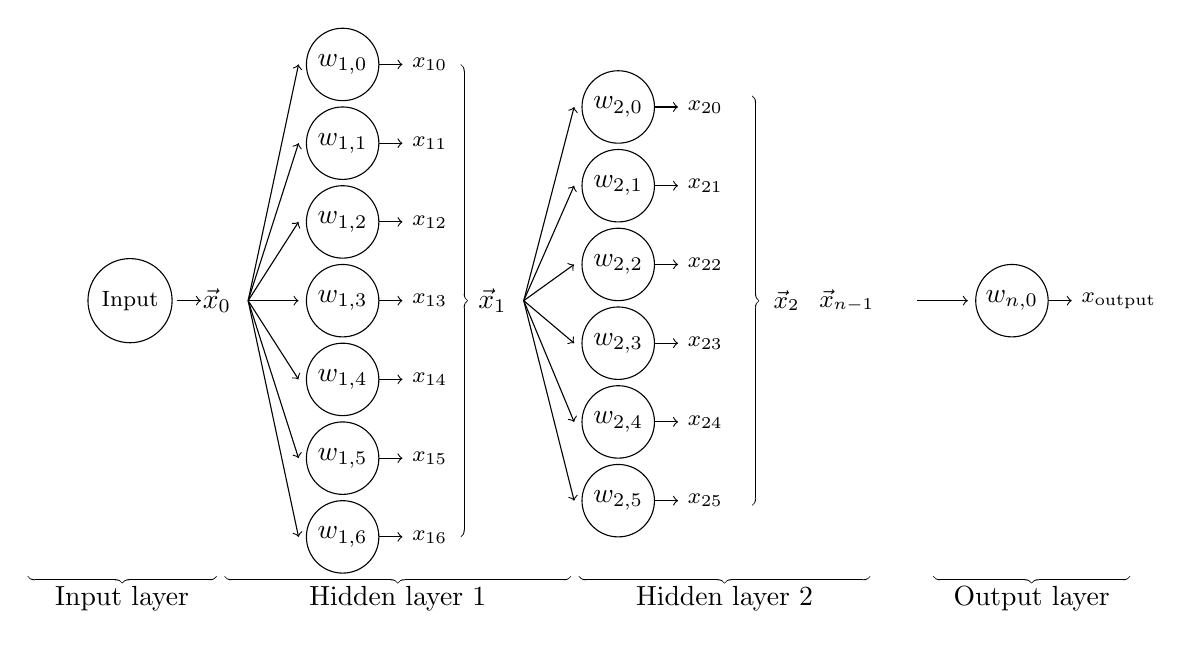
\begin{tikzpicture}
			% \draw (0,0) circle (0.4);
			\pause\node[draw,circle] at (0.3,0) {\footnotesize Input};
			\draw[->] (0.9,0)--(1.2,0);
			\def\baseheight{-3.5}
			\draw [decorate, decoration = {calligraphic brace}] (1.4,\baseheight) --node[below]{Input layer}  (-1,\baseheight);
			\node[anchor=west] at (1.1,0) {$\vec{x}_0$};

			\pause
			
			
			% \draw [decorate, decoration = {calligraphic brace}] (1.3,1.2) --  (1.3,-1.2);
			
			\foreach \i[count=\j from 0] in {3,2,...,-3}
			{
				\def\r{0.46}
				\def\y{\i}
				\def\x{3}
				\draw[->] (1.8,0)--({\x-\r-0.1},\y);
				\draw (\x,{\y}) circle ({\r});
				\node at (\x,{\y}) { $\cec{w}_{1,\j}$};
				\draw [->] ({\x+\r},{\y})--({\x+\r+0.3},{\y});
				\def\xx{\x+\r+0.3}
				% \draw[fill=white] ({\x-\r},{\y-\r})--({\x+\r},{\y-\r})--({\x+\r},{\y+\r})--({\x-\r},{\y+\r})--cycle;
				\node[anchor=west] at (\xx,{\y}) {\fontsize{8}{0}\selectfont$x_{1\j}$};%\phi_{1}^{\j}(y_{1}^{\j})$};
			}
			\pause\draw [decorate, decoration = {calligraphic brace}] (4.5,3) --  (4.5,-3);
			\node[anchor=west] at (4.6,0) {$\vec{x}_1$};
			\pause\draw [decorate, decoration = {calligraphic brace}] (5.9,\baseheight) --node[below]{Hidden layer 1}  (1.5,\baseheight);
			
			\pause

			\foreach \i[count=\j from 0] in {2,1,0,-1,-2,-3}
			{
				\def\r{0.46}
				\def\y{\i+\r}
				\def\x{6.5}
				\draw[->] (5.3,0)--({\x-\r-0.1},\y);
				\draw (\x,{\y}) circle ({\r});
				\node at (\x,{\y}) { $\cec{w}_{2,\j}$};
				\draw [->] ({\x+\r},{\y})--({\x+\r+0.3},{\y});
				\def\xx{\x+\r+0.3}
				% \draw[fill=white] ({\x-\r},{\y-\r})--({\x+\r},{\y-\r})--({\x+\r},{\y+\r})--({\x-\r},{\y+\r})--cycle;
				\node[anchor=west] at (\xx,{\y}) {\fontsize{8}{0}\selectfont$x_{2\j}$};%\phi_{2}^{\j}(y_{2}^{\j})$};
			}
			\draw [decorate, decoration = {calligraphic brace}] (8.2,2.6) --  (8.2,-2.6);
			\draw [decorate, decoration = {calligraphic brace}] (9.7,\baseheight) --node[below]{Hidden layer 2}  (6,\baseheight);
			\node[anchor=west] (A) at (8.35,0) {\small$\vec{x}_2$};
			\pause\node[anchor=west] at (A.east) {\small$\hdots\vec{x}_{n-1}$};
			\pause\foreach \i[count=\j from 0] in {0}
			{
				\def\r{0.46}
				\def\y{\i}
				\def\x{11.5}
				\draw[->] (10.3,0)--({\x-\r-0.1},\y);
				\draw (\x,{\y}) circle ({\r});
				\node at (\x,{\y}) { $\cec{w}_{n,\j}$};
				\draw [->] ({\x+\r},{\y})--({\x+\r+0.3},{\y});
				\def\xx{\x+\r+0.3}
				% \draw[fill=white] ({\x-\r},{\y-\r})--({\x+\r},{\y-\r})--({\x+\r},{\y+\r})--({\x-\r},{\y+\r})--cycle;
				\node[anchor=west] at (\xx,{\y}) {\fontsize{8}{0}\selectfont$x_\text{output}$};
			}
			
			\draw [decorate, decoration = {calligraphic brace}] (13,\baseheight) --node[below]{Output layer}  (10.5,\baseheight);
			% \draw [decorate, decoration = {calligraphic brace}] (15,1) --  (15,-1);
			% \node[anchor=west] at (15.2,0) {$\vec{x}_{n}$};
		\end{tikzpicture}
	\end{frame}
	}
	\begin{frame}{The Multilayered Perceptron}
		Perfect, right?

		\pause 
		\begin{equation}
			x_{10} = \sum_{i} \left[\vec{w}_{1,0}\right]_i \left[ \vec{x}_0\right]_i \LLR \vec{x}_1 = W_1 \vec{x}_0
		\end{equation}
		\pause And therefore:
		\begin{equation}
			\vec{x}_n = \left(\prod_{j=1}^n W_j \right) \vec{x}_0
		\end{equation}

		\pause Just one giant matrix product: still fundamentally linear! 

		\pause For our `cute' problem, even a 10,000 layer network with 5 million nodes will ultimately reduce into a single $2\times 1$ matrix (i.e. a single dot product).
	\end{frame}

	\begin{frame}{Breaking Linearity}
		Introduce the idea of `activation functions':
		\begin{equation}
			x_{n,i} = \phi\left( \vec{w}_{n,i} \cdot \vec{x}_{n-1} \right)
		\end{equation}

		$\phi$ has following properties:
		\begin{itemize}
			\pitem A simple 1:1 function
			\pitem Non-linear
			\pitem Works on each element of the vector individually
		\end{itemize}

		\pause In practice, we like some other properties (analytical derivatives, easy to compute etc.)
	\end{frame}
	\begin{frame}{Activation Functions}
		Some common choices:
		\begin{itemize}
			\pitem Rectified Linear Unit (ReLU)
			$$ \phi(x) = \begin{cases} x &\text{ when } x > 0 \\ 0 &\text{else} \end{cases}$$
			\pitem  Leaky ReLU
			$$ \phi(x) = \begin{cases} x &\text{ when } x > 0 \\ 0.01x &\text{else} \end{cases}$$
			\pitem Sigmoid
			$$ \phi(x) = \frac{1}{1 + e^{-x}} $$
			\pitem Softplus
			$$ \phi(x) = \ln\left( 1 + e^x \right)$$
		\end{itemize}
		% \pause Except at the output layer, the choice of node must be chosen on an empirical basis!
	\end{frame}
	
	{
	\nologo
	\begin{frame}{The Multilayered Perceptron}
		% Let's try chaining lots of pecreptrons together.....
		
		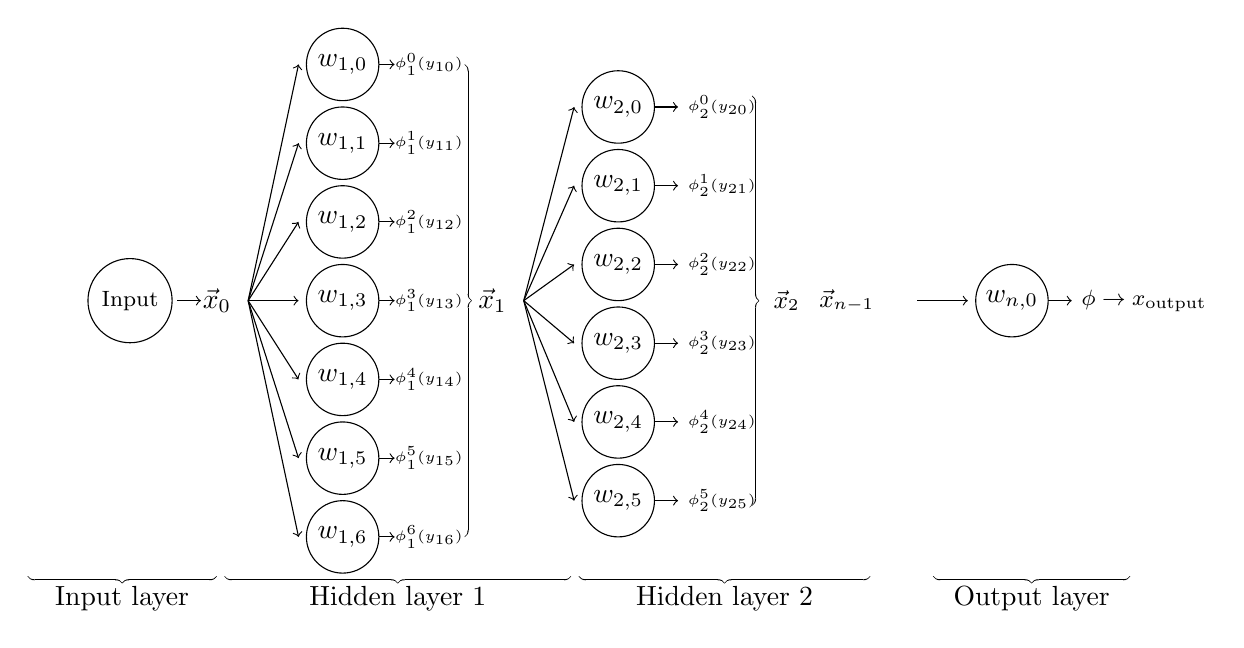
\begin{tikzpicture}
			% \draw (0,0) circle (0.4);
			\pause\node[draw,circle] at (0.3,0) {\footnotesize Input};
			\draw[->] (0.9,0)--(1.2,0);
			\def\baseheight{-3.5}
			\draw [decorate, decoration = {calligraphic brace}] (1.4,\baseheight) --node[below]{Input layer}  (-1,\baseheight);
			\node[anchor=west] at (1.1,0) {$\vec{x}_0$};

			\pause
			
			
			% \draw [decorate, decoration = {calligraphic brace}] (1.3,1.2) --  (1.3,-1.2);
			
			\foreach \i[count=\j from 0] in {3,2,...,-3}
			{
				\def\r{0.46}
				\def\y{\i}
				\def\x{3}
				\draw[->] (1.8,0)--({\x-\r-0.1},\y);
				\draw (\x,{\y}) circle ({\r});
				\node at (\x,{\y}) { $\cec{w}_{1,\j}$};
				\draw [->] ({\x+\r},{\y})--({\x+\r+0.2},{\y});
				\def\xx{\x+\r+0.08}
				% \draw[fill=white] ({\x-\r},{\y-\r})--({\x+\r},{\y-\r})--({\x+\r},{\y+\r})--({\x-\r},{\y+\r})--cycle;
				\node[anchor=west] at (\xx,{\y}) {\fontsize{5}{0}\selectfont$\phi_1^\j(y_{1\j})$};%\phi_{1}^{\j}(y_{1}^{\j})$};
			}
			\pause\draw [decorate, decoration = {calligraphic brace}] (4.55,3) --  (4.55,-3);
			\node[anchor=west] at (4.6,0) {$\vec{x}_1$};
			\pause\draw [decorate, decoration = {calligraphic brace}] (5.9,\baseheight) --node[below]{Hidden layer 1}  (1.5,\baseheight);
			
			\pause

			\foreach \i[count=\j from 0] in {2,1,0,-1,-2,-3}
			{
				\def\r{0.46}
				\def\y{\i+\r}
				\def\x{6.5}
				\draw[->] (5.3,0)--({\x-\r-0.1},\y);
				\draw (\x,{\y}) circle ({\r});
				\node at (\x,{\y}) { $\cec{w}_{2,\j}$};
				\draw [->] ({\x+\r},{\y})--({\x+\r+0.3},{\y});
				\def\xx{\x+\r+0.3}
				% \draw[fill=white] ({\x-\r},{\y-\r})--({\x+\r},{\y-\r})--({\x+\r},{\y+\r})--({\x-\r},{\y+\r})--cycle;
				\node[anchor=west] at (\xx,{\y}) {\fontsize{5}{0}\selectfont$\phi_2^\j(y_{2\j})$};%\phi_{2}^{\j}(y_{2}^{\j})$};
			}
			\draw [decorate, decoration = {calligraphic brace}] (8.2,2.6) --  (8.2,-2.6);
			\draw [decorate, decoration = {calligraphic brace}] (9.7,\baseheight) --node[below]{Hidden layer 2}  (6,\baseheight);
			\node[anchor=west] (A) at (8.35,0) {\small$\vec{x}_2$};
			\pause\node[anchor=west] at (A.east) {\small$\hdots\vec{x}_{n-1}$};
			\pause\foreach \i[count=\j from 0] in {0}
			{
				\def\r{0.46}
				\def\y{\i}
				\def\x{11.5}
				\draw[->] (10.3,0)--({\x-\r-0.1},\y);
				\draw (\x,{\y}) circle ({\r});
				\node at (\x,{\y}) { $\cec{w}_{n,\j}$};
				\draw [->] ({\x+\r},{\y})--({\x+\r+0.3},{\y});
				\def\xx{\x+\r+0.3}
				% \draw[fill=white] ({\x-\r},{\y-\r})--({\x+\r},{\y-\r})--({\x+\r},{\y+\r})--({\x-\r},{\y+\r})--cycle;
				\node[anchor=west] at (\xx,{\y}) {\fontsize{8}{0}\selectfont$\phi\to x_\text{output}$};
			}
			
			\draw [decorate, decoration = {calligraphic brace}] (13,\baseheight) --node[below]{Output layer}  (10.5,\baseheight);
			% \draw [decorate, decoration = {calligraphic brace}] (15,1) --  (15,-1);
			% \node[anchor=west] at (15.2,0) {$\vec{x}_{n}$};
		\end{tikzpicture}
	\end{frame}
	}

	\begin{frame}{Training}
		\begin{itemize}
			\pitem `Training' is about finding the set $\{ \vec{w}_{ij} \}$ which produce the most accurate predictions
			\pitem It is an \textit{optimisation} problem 
		\end{itemize}

		\pause Naive optimisation function ($L_2$ cost function):
		\begin{equation}
			\mathcal{L}(\{ \vec{w}_{ij} \}) = \sum_{q \text{ in dataset}} \left(\mathcal{P}(\vec{x}_q | \{ \vec{w}_{ij} \}) - L_q\right)^2
		\end{equation}
		\pause Big when $\mathcal{P} \neq L$, small when $\mathcal{P} = L ~~\to$  need to \textit{minimise} this function
	\end{frame}

	\begin{frame}{Optimisation}
		
		\begin{center}
		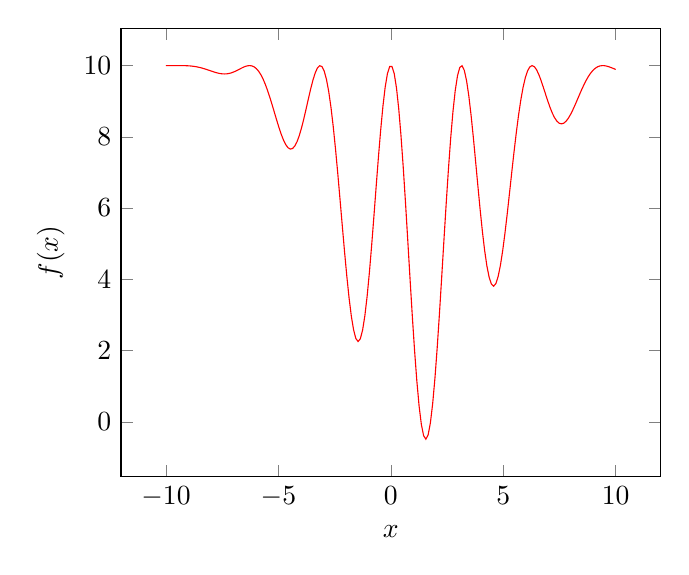
\begin{tikzpicture}
			\begin{axis}[xlabel = \(x\),
				ylabel = {\(f(x)\)}]
			\addplot[color=red,domain=-10:10,samples=200]{10 - ((exp(-(x/5)^2) * (sin(x * 180/3.141592654))^2)*(x+10))};
			\end{axis}
			\end{tikzpicture}
		\end{center}
		\pause What value of $x$ has lowest value of $f(x)$?
	\end{frame}

	\begin{frame}{Optimisation}
		\pause Easy in 1D:
		\begin{itemize}
			\pitem If $\div{y}{x}$ computable, then $\div{^2 y}{x^2}$ etc. 
			\pitem 400 years of support!
		\end{itemize}

		\pause In higher dimensions....gets very tricky:
		\begin{itemize}
			\pitem First order derivative, $\nabla y(\vec{x})$, has $n$ components
			\pitem Second order methods require inverting $H_{ij} = \pdiv{^2y}{x_i \partial x_j}$
			\pitem Theoretical solutions not \textbf{practical}
		\end{itemize}

		
	\end{frame}

	\begin{frame}{Optimisers}
		\pause Simple MLPs have $>1000s$ parameters -- squarely in the high dimensional space!

		\pause We therefore use 'dumb' first order methods:
		\begin{center}
			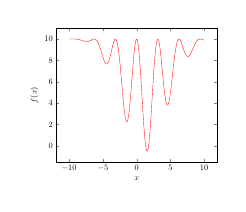
\begin{tikzpicture}[scale=0.3]
				\begin{axis}[xlabel = \(x\),
					ylabel = {\(f(x)\)}]
				\addplot[color=red,domain=-10:10,samples=200]{10 - ((exp(-(x/5)^2) * (sin(x * 180/3.141592654))^2)*(x+10))};
				\end{axis}
				\end{tikzpicture}
			\end{center}
		\begin{enumerate}
			\pitem Start at random network initialisation $w_0$
			\pitem Find gradient $\nabla_w \mathcal{L}$ at current position
			\pitem Take step in (opposite) direction of gradient, update weights
			\pitem Go to 2)
		\end{enumerate}

		\pause Various modifications (adaptive learning, momentum etc.)

		% \pause All optimisers (ADAM, AdaGrad, RMSProp, Line Search) use variations on this basic method
	\end{frame}	

	\begin{frame}{Derivatives of Networks}

		\pause Fundamentally need \textit{derivatives}: in which direction does changing $\{\vec{w}\}$ improve $\mathcal{L}$?

		\begin{equation}
			\mathcal{L}(\{ \vec{w}_{ij} \}) = \sum_{q \text{ in dataset}} \left(\mathcal{P}(\vec{x}_q | \{ \vec{w}_{ij} \}) - L_q\right)^2
		\end{equation}

		\pause But $\mathcal{L}$ is a \textit{complicated} function of $\{\vec{w}\}$! 
	\end{frame}
	\begin{frame}{Chain Rule: Crash Course}
		If $y$ is a function of $x$, and $f$ is a function of $y$, then:
		\begin{equation}
			\div{f}{x} = \div{f}{y} \div{y}{x}
		\end{equation}
		\pause \textit{The rate of change of $f$ with $x$ is the rate at which $y$ changes with $x$, times the rate at which $f$ changes with $y$}

		\pause In higher dimensions, have to sum over all possible combinations:
		\begin{equation}
			\div{f}{x} = \sum_i \pdiv{f}{y_i} \pdiv{y_i}{x}
		\end{equation}
		\pause \textit{The rate of change of $f$ with $x$ is the sum of all of the rates at which $y_i$ changes with $x$, times the rate at which $f$ changes with $y_i$}
	\end{frame}

	\begin{frame}{Back to the optimisation problem}
		$w_{ijk}$ is the $k^\text{th}$ element of weight vector in the $j^\text{th}$ node, in the $i^\text{th}$ layer.
		\begin{equation}
			\pdiv{\mathcal{L}}{w_{ijk}} = \sum_{i \text{ in dataset}} \left(\mathcal{P}(\vec{x}_i | \{ \vec{w}_{ij} \}) - L_i\right) \pdiv{P}{w_{ijk}}
		\end{equation}

		\pause Have two cases: $i$ is the final layer, or it is not. If in the final layer, this is trivial:
		\begin{spalign}
			\mathcal{P} = x_\text{final} & = \phi(\underbrace{\vec{w}_{f} \cdot\vec{x}_{i-1}}_{y_{ij}})
			\\
			\pdiv{P}{\vec{w}_{ij}} & = \left. \pdiv{\phi}{y} \right|_{y =y_{ij} } \vec{x}_{i-1}
			\\
			& = \phi^\prime (y_{ij}) \vec{x}_{n-1}
		\end{spalign}
		\pause Therefore:
		\begin{equation}
			\pdiv{\mathcal{L}}{w_{\text{final}  k}} = \sum_{i \text{ in dataset}} \left(\mathcal{P}(\vec{x}_i | \{ \vec{w}_{ij} \}) - L_i\right) \phi^\prime(y_\text{final}) \left[\vec{x}_{i-1}\right]_k
		\end{equation}
	\end{frame}
	\begin{frame}{What about non-final layers?}
		Consider:
		\pause
		\begin{spalign}
			\vec{x}_{i} & = \begin{pmatrix} \phi(\vec{x}_i \cdot \vec{w}_{i,0}) \\  \phi(\vec{x}_{i-1} \cdot \vec{w}_{i,1}) \\ \vdots \\  \phi(\vec{x}_{i-1} \cdot \vec{w}_{i,j}) \end{pmatrix}\pause = \begin{pmatrix} \phi(y_{i,0} \\ \phi(y_{i,1}) \\ \vdots \\ \phi(y_{i,j})) \end{pmatrix}
		\end{spalign}
		\pause By the chain rule:
		\begin{spalign}
			\pdiv{\mathcal{L}}{w_{ijk}} & = \pdiv{\mathcal{L}}{y_{ij}} \pdiv{y_{ij}}{w_{ijk}}
			\\
			& = \pdiv{\mathcal{L}}{y_{ij}} \left[\vec{x}_{i-1} \right]_k
		\end{spalign}

	\end{frame}
	\begin{frame}{Almost there....}
		Finally, we note that $\pdiv{\mathcal{L}}{y_{i+1,j}}$ is simply a statement about how changing $y$ (the dot product) alters $L$, but that via the chain rule again:
		\begin{equation}
			\pdiv{\mathcal{L}}{y_{ij}} = \sum_{p \text{ nodes in next layer}} \pdiv{\mathcal{L}}{y_{i+1,p}} \pdiv{y_{i+1,p}}{y_{ij}}
		\end{equation}
		\pause \textit{The rate of change of L with respect to $y_{ij}$ is equal to the sum of rates at which $y_{ij}$ changes $y_{i+1,p}$ in the next layer, multiplied by how $y_{i+1,p}$ changes $\mathcal{L}$ }
	\end{frame}

	\begin{frame}{Backpropagation}
		\pause How does this help?

		\pause We go \textit{backwards} through the network. Start at the final layer:
		\begin{spalign}
			\pdiv{\mathcal{L}}{y_{\text{final}}} = \phi^\prime(y_\text{final}) 
		\end{spalign}
		
		\pause Then feed this into the next layer down:
		\begin{spalign}
			\pdiv{\mathcal{L}}{y_{\text{final} -1,j}} = \phi^\prime(y_{\text{final}-1}) \pdiv{\mathcal{L}}{y_{\text{final}}} w_\text{final,j}
		\end{spalign}

		\pause And so on...

		\pause This is \textbf{backpropagation}: a fancy way of using the chain rule
	\end{frame}

	\begin{frame}{And....you're done!}
		\begin{center}
			\LARGE
			This is all you need
			\\
			\pause Let's see it in action!
		\end{center}
	\end{frame}
\end{document}